\chapter{Results}\label{section:results}

    Here we present the results from our two different experiments.

    We compare the results of our code-prose experiment to the original study~\cite{floyd_decoding_2017} and the replication study~\cite{fucci_replication_2019}, and investigate the results from our naturalistic device use experiment to see if results generalize to other types of device activity.

    \change[inline]{Update with final values}

    \section{Code vs prose task}
        Table~\ref{table:bac-all} shows the BAC scores for the code vs prose task.

        The \emph{Benchmark} columns show show the results for the 8 subjects using the bandpower benchmark for window-level data and epoch-level data, respectively. Analogously, the \emph{Riemannian} columns show the corresponding results using Riemannian geometry. The classifier using Riemann geometry outperforms the baseline by TODO.

        Our top-performing classifier, using LORO cross-validation, yields a median BAC score of $0.749$  for window-level classification and $0.9$ for epoch-level classification (seen in Table~\ref{table:bac-selective}).

        The top-performing classifier computes the covariance matrices, and then uses using Riemannian geometry, Common Spatial Pattern, and TangentSpace. With logistic regression for the final step.

        We do window-level classification by training on the \SI{5}{\second} windows (as described in Section~\ref{section:transform}).

        We achieve epoch-level classification by training a window-level classifier just as for the \SI{5}{\second} windows, we then make a classification for the entire epoch by taking the mean of the prediction probabilities from the windows in that epoch.

        \add[inline]{Markus: Vilken modell är det som gäller nu? Och vilka features och clearning och sånt bygger den på? Kanske avsluta kapitel 3 med att tydligt presentera vad som används i experimenten?}
        
        \begin{comment}
            The following is the performance statistics for our model trained on \SI{5}{\second} windows. It is trained on all subjects except one, which is used in testing:

            \begin{verbatim}
            INFO: {
                'precision': 0.7473868367437329, 
                'recall': 0.696405129166862, 
                'fbeta': 0.6703482474923927, 
                'support': array([308, 277]), 
                'bac': 0.696405129166862, 
                'confusion_matrix': array([[141, 167], [ 18, 259]])
            }
            \end{verbatim}

            The following are the performance statistics for our model on the epoch-level.  The same subject selection as the previous statistics is used:

            \begin{verbatim}
            INFO: {
                'precision': 0.8541666666666667, 
                'recall': 0.7666666666666666, 
                'fbeta': 0.7624602332979852, 
                'support': array([15, 17]), 
                'bac': 0.7666666666666666, 
                'confusion_matrix': array([[ 8,  7], [ 0, 17]])
            }
            \end{verbatim}
        \end{comment}

        \begin{table}[h]
            \centering
            \begin{tabular}{lcccc}
                \toprule
                & \multicolumn{2}{c}{\textbf{Riemannian}} & \multicolumn{2}{c}{\textbf{Bandpower}} \\
                \cmidrule(lr){2-3}
                \cmidrule(lr){4-5}
                \textbf{Subject} & Window-level & Epoch-level & Window-level & Epoch-level \\
                \midrule
                \#0  & 0.608  & 0.603 & x & x \\
                \#1  & 0.802  & 0.864 & x & x \\
                \#5  & 0.589  & 0.534 & x & x \\
                \#6  & 0.701  & 0.767 & x & x \\
                \#7  & 0.694  & 0.8   & x & x \\
                \#8  & 0.547  & 0.542 & x & x \\
                \#9  & 0.484  & 0.5   & x & x \\
                \#10 & 0.474  & 0.5   & x & x \\
                \midrule
                Median & 0.5985 & 0.573 & x & x \\
                \bottomrule
            \end{tabular}
            \caption{The BAC score for each LORO fold/subject. Excluding subjects 3 and 4.}\label{table:bac-all}
        \end{table}

        In Table~\ref{table:bac-all} we see that performance is bad (no better than chance) for several subjects. We investigate these and find issues with the amount of data (and\ldots). We remove them from analysis, and get the much improved results in Table~\ref{table:bac-selective}.

        We discuss our subject selection further in Section~\ref{section:discussion}.

        \begin{table}[h]
            \centering
            \begin{tabular}{lcccc}
                \toprule
                & \multicolumn{2}{c}{\textbf{Riemannian}} & \multicolumn{2}{c}{\textbf{Bandpower}} \\
                \cmidrule(lr){2-3}
                \cmidrule(lr){4-5}
                \textbf{Subject} & Window-level & Epoch-level & Window-level & Epoch-level \\
                \midrule
                \#0 & 0.673 & 0.727 & 0.533 & 0.551 \\
                \#1 & 0.895 & 0.955 & 0.687 & 0.859 \\
                \#5 & 0.616 & 0.542 & 0.614 & 0.792 \\
                \#6 & 0.864 & 0.908 & 0.730 & 0.808 \\
                \#7 & 0.749 & 0.9   & 0.634 & 0.733 \\
                \midrule
                Median & 0.749 & 0.9 & 0.634 & 0.792 \\
                \bottomrule
            \end{tabular}
            \caption{The BAC score for each LORO fold/subject. Excluding subjects 3, 4, 8, 9, and 10.}\label{table:bac-selective}
        \end{table}

        \begin{comment}
            \begin{table}
                \begin{center}
                    \begin{tabular}{lcc}
                        \toprule
                                & Window-level & Epoch-level \\
                        \midrule
                        Precision & 74.7\% & 85.4\%  \\
                        BAC       & 69.6\% & 76.7\%  \\
                        \bottomrule
                    \end{tabular}
                    \caption{Performance statistics of our models trained on all subjects with good signal quality except number \#6, which is used for testing.}\label{fig:stats}
                \end{center}
            \end{table}
        \end{comment}


        \change[inline]{Remove excessive bars (quality? train/test split? predicted (prob)?). Explain meaning of colors. Update with version that has subjects numbered.}
        \begin{landscape}
            \begin{figure}
                \centering
                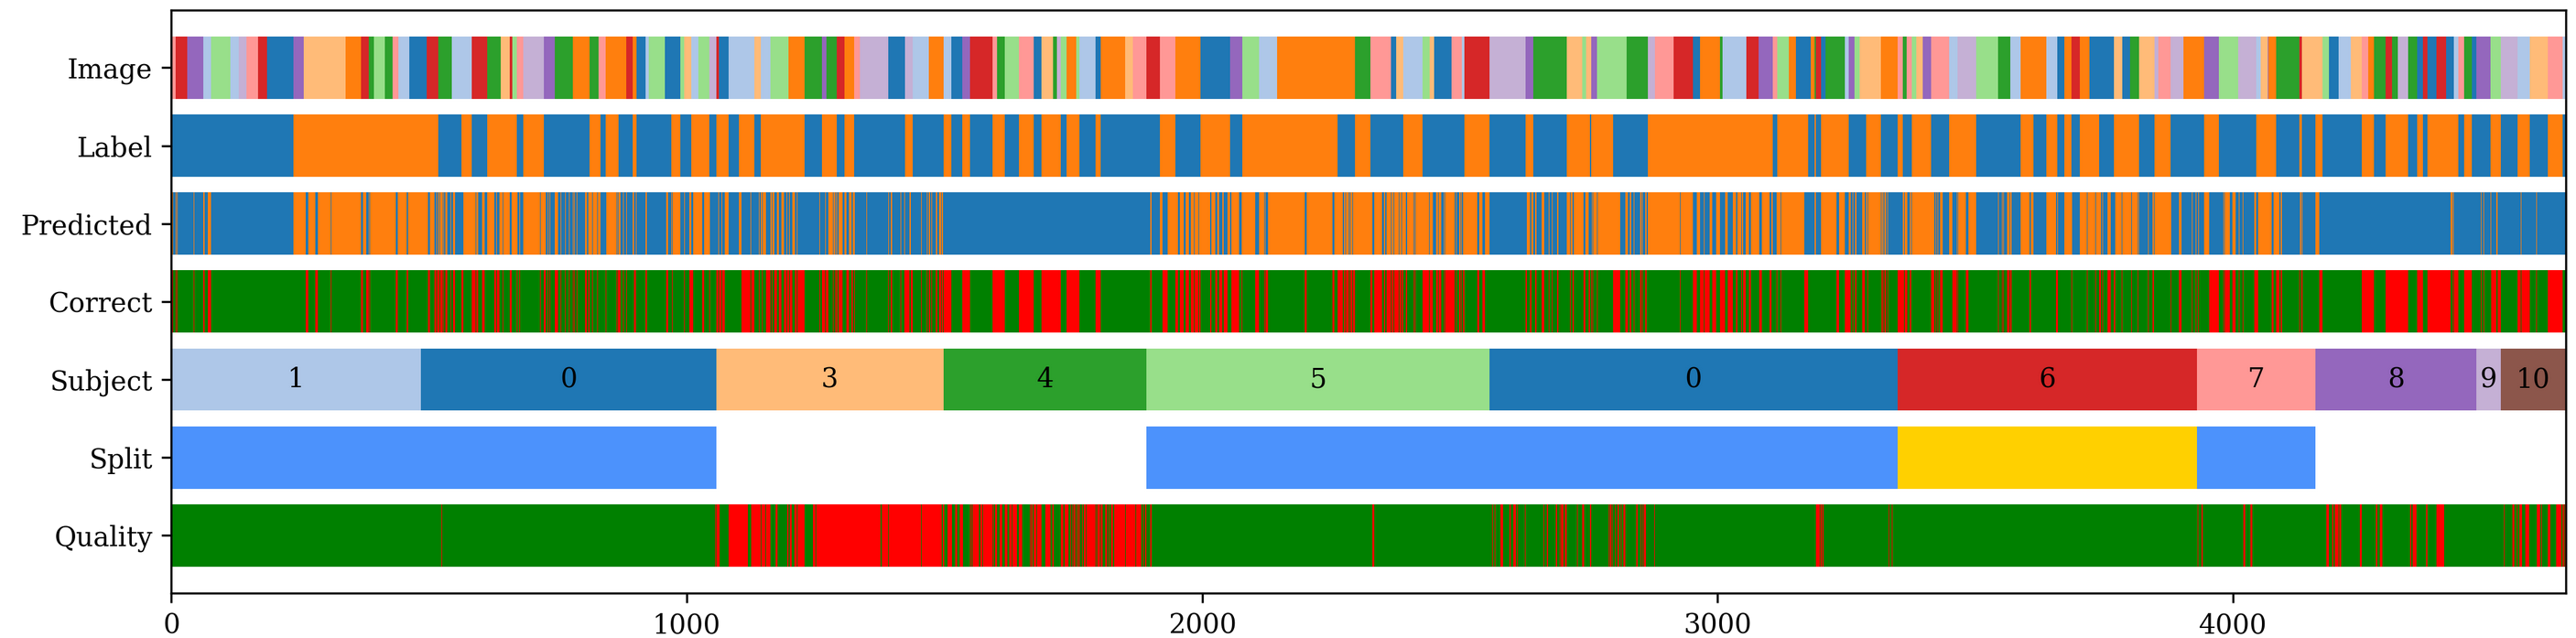
\includegraphics[width=24cm]{img/timebars.png}
                \caption{Visualization of the labeled data with classifications from one fold. Shows the \emph{Image} (stimuli), the \emph{Label} for that stimuli, the \emph{Predicted} class, whether the prediction is \emph{Correct}, the \emph{Subject}, the \emph{Split}/Fold, and our threshold measure for signal \emph{Quality}. The x-axis is the window index, sorted by acquisition time.
                \\
                \\
                It can be seen that (1) subjects \#3 and \#4 have bad signal quality, and have therefore been excluded from the training set. (2) The subjects \#9 and \#10 have also been excluded from training due to issues during data collection. (3) For subject \#1 the stimuli images were not shuffled. (4) Subject \#0 appears twice, as they did two sessions (using unseen stimuli).}\label{fig:timebars}
            \end{figure}
        \end{landscape}

        \begin{comment}
            \begin{figure}[h]
            \centering
            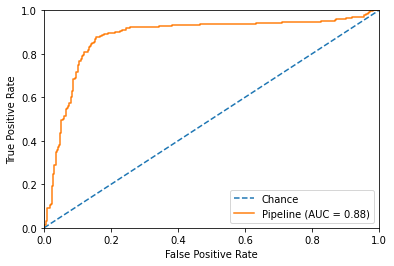
\includegraphics[width=12cm]{img/roccurve.png}
            \caption{Receiver operating characteristic (ROC) curve for subject \#6.}\label{fig:roc}
            \end{figure}
            \change[inline]{Update with higher-res image}
        \end{comment}

        Compared to previous studies, we achieve a moderate improvement over the EEG-only classifier trained in Fucci et al., and achieve a similar performance to the fMRI study by Floyd et al. (seen in Table~\ref{table:compare-results}).

        \begin{table}
            \begin{center}
                \begin{tabular}{lccc}
                    \toprule
                    & \textbf{This study} & \textbf{Fucci et al.} & \textbf{Floyd et al.} \\
                    \midrule
                    Overall & 0.75 & 0.66 & 0.79 \\
                    Code & x & x & x \\
                    Prose & x & x & x \\
                    \bottomrule
                \end{tabular}
                \caption{Result comparison between the previous studies and this study. Best BAC results are reported. For Fucci et al.\ we chose the best EEG-only score.}\label{table:compare-results}
            \end{center}
        \end{table}

    \section{Naturalistic device activity}

        We collected $\sim5$ hours of labeled EEG data during natural device use.

        We use the classes defined in Section~\ref{section:collect-usage}.

        We train classifiers for the label pairs:

        \begin{itemize}
                \item Programming / Writing
                \item Programming / Twitter
                \item Twitter / YouTube
        \end{itemize}

        Our results are seen in Table~\ref{table:scores-natural}.

        \begin{table}[h]
            \centering
            \begin{tabular}{llrr}
                \toprule
                Experiment & Score & Support & Hours of data \\
                \midrule
                Programming vs Writing & 0.676 & (1386, 209) & 2.22h \\
                Programming vs Twitter & 0.695 &  (1386, 949) & 3.24h \\
                Twitter vs YouTube & 0.604 & (949, 266) & 1.69h \\
                \bottomrule
            \end{tabular}
            \caption{The scores for each label pairing. The score is the mean BAC of the StratifiedKFold splits.}\label{table:scores-natural}
        \end{table}

        The class distribution is as follows: TODO
